% Cal Poly Thesis
% 
% based on UC Thesis format
%
% modified by Mark Barry 2/07.
%

\documentclass[12pt]{ucthesis}

\usepackage{amssymb}
\usepackage{amsmath}
\usepackage[letterpaper]{geometry}
\usepackage[overload]{textcase}
\usepackage{enumitem}
\usepackage{listings}
\usepackage{ifpdf}
\ifpdf
    \usepackage[pdftex]{graphicx}
    \graphicspath{ {./images/} }
    % Update title and author below...
    \usepackage[pdftex,plainpages=false,pdfpagelabels,breaklinks=true,colorlinks=true,urlcolor=blue,citecolor=blue,%
                                       linkcolor=blue,bookmarks=true,bookmarksopen=true,%
                                       bookmarksopenlevel=3,pdfstartview=FitV,
                                       pdfauthor={Alexander Paul Sideropoulos},
                                       pdftitle={dCAMP: Distributed Common API for Measuring Performance},
                                       pdfkeywords={thesis, masters, cal poly, distributed computing, performance monitoring}
                                       ]{hyperref}
    %Options with pdfstartview are FitV, FitB and FitH
    \pdfcompresslevel=1
\else
    \usepackage{graphicx}
\fi

% no line spacing with lists
\setlist{nolistsep}

\setlength{\parindent}{0.25in} \setlength{\parskip}{6pt}

\geometry{verbose,nohead,tmargin=1.25in,bmargin=1in,lmargin=1.5in,rmargin=1.3in}

\setcounter{tocdepth}{2}

% Different font in captions (single-spaced, bold) ------------
\newcommand{\captionfonts}{\small\bf\ssp}

\makeatletter  % Allow the use of @ in command names
\long\def\@makecaption#1#2{%
  \vskip\abovecaptionskip
  \sbox\@tempboxa{{\captionfonts #1: #2}}%
  \ifdim \wd\@tempboxa >\hsize
    {\captionfonts #1: #2\par}
  \else
    \hbox to\hsize{\hfil\box\@tempboxa\hfil}%
  \fi
  \vskip\belowcaptionskip}
\makeatother   % Cancel the effect of \makeatletter
% ---------------------------------------

%custom commands
\newcommand{\camp}{\emph{CAMP }}
\newcommand{\dcamp}{\emph{dCAMP }}

\begin{document}

% Declarations for Front Matter

% Update fields below!
\title{dCAMP: Distributed Common API for Measuring Performance}
\author{Alexander Paul Sideropoulos}
\degreemonth{June} \degreeyear{2014} \degree{Master of Science}
\defensemonth{June} \defenseyear{2014}
\numberofmembers{3} \chair{Dr. Michael Haungs} \othermemberA{Dr. Gene Fisher} \othermemberB{Dr. David Janzen} \field{Computer Science} \campus{San Luis Obispo}
\copyrightyears{seven}

\maketitle

\begin{frontmatter}

% Custom made for Cal Poly (by Mark Barry).
\copyrightpage

% Custom made for Cal Poly (by Andrew Tsui).
\committeemembershippage

\begin{abstract}

Although the nearing end of Moore's Law has been predicted numerous times in the past \cite{schaller1997}, it will eventually come to pass. In forethought of this, many modern computing systems to become increasingly complex, distributed, and parallel. As software is developed on and for these complex systems, a common API is necessary for gathering vital performance related metrics while remaining transparent to the user, both in terms of system impact and ease of use. Several distributed performance monitoring and testing systems have been proposed and implemented by both research and commercial institutions. However, most of these systems do not meet several fundamental criterion for a truly useful distributed performance monitoring system: 1) variable data delivery models, 2) security, 3) scalability, 4) transparency, 5) completeness, 6) validity, and 7) portability \cite{zanikolas2005}. This work presents the Distributed Common API for Measuring Performance, \dcamp, as a solution to meet each of these criterion.

\end{abstract}



\begin{acknowledgements}

   Thank you...

\end{acknowledgements}

\addcontentsline{toc}{chapter}{Contents}
\tableofcontents

\listoftables
\listoffigures

\end{frontmatter}

\pagestyle{plain}

\renewcommand{\baselinestretch}{1.66}

% ------------- Main chapters here --------------------

\chapter{Introduction}
\label{introduction}

As the Internet has become more pervasive in today's business economy, there has been a natural trend of distributing
large, complex systems across multiple components locally and throughout the world. These systems are not always
homogeneous with respect to hardware architecture or even operating system, and development of these system can prove to
be quite difficult even with the best tools available. In order to effectively build these systems, software engineers
must be able to test their system for performance defects as well as bottlenecks. Additionally, distributed systems must
respond to changes in availability and work load on its individual nodes.

Distributed performance testing frameworks supply software practitioners and system administrators with tools to
evaluate the performance of a system from both black box and white box perspectives by publishing interfaces for
instrumenting, collecting, analyzing, and visualizing performance data across the distributed system and distributed
applications. Distributed performance monitoring frameworks, often considered part of the testing framework, provide a
black box interface into monitoring a distributed system or application and usually includes mechanisms for triggering
actions based on performance events. For the purpose of this work, the term distributed performance framework is
introduced to collectively refer to both distributed performance testing and distributed performance monitoring
frameworks.

\section{Distributed Performance Framework Criterion}

In order for practitioners and researchers alike to effectively choose a distributed performance framework, it is
necessary to have a set criteria for evaluation. Presented here is an extended criterion of the general requirements
presented by \cite{zanikolas2005} for grid systems. Data Delivery Models and Security have been taken directly from
their work. Scalability has been modified to only consider good performance as its goal while Low Intrusiveness has been
turned into Transparency. Extensibility has been removed from the list, and Completeness and Validity have been added.
This work provides an alternate definition for Portability.

\subsubsection{Data Delivery Models}

Monitoring information includes fairly static (e.g., software and hardware configuration of a given node) and dynamic
events (e.g., current processor load, memory), which suggests the use of different measurement policies (e.g., periodic
or on demand). In addition, consumer patterns may vary from sparse interactions to long lived subscriptions for
receiving a constant stream of events. In this regard, the monitoring system must support both pull and push data
delivery models.
\cite{zanikolas2005}

\subsubsection{Security}

Certain scenarios may require a monitoring service to support security services such as access control, single or mutual
authentication of parties, and secure transport of monitoring information.
\cite{zanikolas2005}

\subsubsection{Scalability}

Monitoring systems have to cope efficiently with a growing number of resources, events and users. This scalability can
be achieved as a result of good performance which guarantees that a monitoring system will achieve the needed throughput
within an acceptable response time in a variety of load scenarios.
\cite{zanikolas2005}

\subsubsection{Transparency}

Transparency refers to the lack of impact a distributed performance framework makes on the system being monitored. As
\cite{zanikolas2005} states, it is ``typically measured as a function of host (processor, memory, I/O) and network load
(bandwidth) generated by the collection, processing and distribution of events.'' If a framework lacks transparency it
will fail to allow the underlying distributed system to perform well and will produce inaccurate performance
measurements, thereby reducing its Scalability and destroying its Validity.

\subsubsection{Completeness}

The Completeness of a distributed performance framework refers to the exhaustiveness to which it gathers performance
metrics. At a minimum, a framework must provide interfaces for measuring and aggregating performance data about a
system's processor, memory, disk, and network usage. Several distributed performance frameworks provide further detailed
performance metrics about the given distributed system being monitored, but this is usually at the cost of Portability.

\subsubsection{Validity}

A distributed performance framework is only as good as the data is produces; if the sensors or gathering techniques are
inaccurate, then the data is useless at best, misleading at worst. Validity of a framework is achieved when the authors
of a framework provide formal verification of its accuracy.

\subsubsection{Portability}

A framework's ability to run on a completely heterogeneous distributed system without special considerations by the
practitioner is what this work defines as Portability. More specifically, a portable framework has a unified API
regardless of the system architecture, does not restrict itself to applications written in specific programming
languages, and does not require practitioners to manually instrument their application code. This black box
characteristic is vital for a viable distributed performance framework's effectiveness as it allows practitioners to
focus on the performance data and not on a myriad of APIs for various architectures or languages.

\section{\dcamp}
\label{dcamp}

The Distributed Common API for Measuring Performance (\dcampns) is a distributed performance framework built on top of
Mark Gabel and Michael Haungs' 2007 research on \emph{CAMP: a common API for measuring performance} \cite{gabel2007}.
The fundamental functionality of \camp is providing an accurate and ``consistent method for retrieving system
performance data from multiple platforms.''

\dcamp takes advantage of this functionality and the authors' work done in validating \campns's accuracy and adds the
core feature sets listed below. As shown in the analysis work presented in Chapter \ref{analysis}, \dcamp adds these
features while still maintaining minimal impact on the systems, processes, and networks being monitored.

The key contributions of the Distributed Common API for Measuring Performance are:

\begin{itemize}
\item a stateful performance API,
\item distributed performance data aggregation,
\item performance filters and triggers, and
\item simplistic fault tolerance.
\end{itemize}

\subsection{Terminology}
Knowing the following terminology will make it easier to understand and discuss the \dcamp project, its main goals, its
usage, its components, and its inner workings. 

\begin{description}

\item[Distributed Performance Testing Framework (DPTF),]
\item[Distributed Performance Monitoring Framework (DPMF),]
\item[Distributed Performance Framework (DPF):]

An DPTF or DPMF (collectively termed DPF) is a framework which allows its users to evaluate the performance of a system
from both black box and white box perspectives by publishing interfaces for instrumenting, collecting, analyzing, and
visualizing performance data across the distributed system and distributed applications. Typically, the framework
provides a black box interface into monitoring a distributed system or application and includes mechanisms for
triggering actions based on performance events. The \dcamp project is designed to be a DPF. 

\item[Performance Metric,]
\item[Performance Counter:]
Performance metrics are any data about a given node relating to its throughput, capacity, utilization, or latency. In
\dcampns, these are grouped into four different sets of performance metrics---global, network, disk, and
per-process---and a fifth set of inquiry metrics. They are described fully in section \ref{dcamp_metrics}. 

\item[Metric Aggregation:]
Metric aggregation is the process of combining metrics from multiple nodes into a single metric. Performance metrics,
while useful at an individual system granularity, can be rather limited in value for a DPF where the goal is measurement
of the distributed system as a whole. Metric aggregation provides a coarser granularity for the performance metrics,
calculating a sum, average, percent, or any other mathematically relevant operation across multiple nodes in the system. 

\item[Metric Calculation:]
Metric calculation is the process of combining identical metrics from multiple timestamps into a single metric. Various
equations and inputs are used to do this calculation, chosen depending on the type of metric and desired representation;
these equations are listed in Table \ref{tab:metric_types}.

\item[Filter,]
\item[Throttle,]
\item[Threshold:]
Filtering (or throttling or thresholding) provides a mechanism for reducing the amount of data sent between nodes of the
system. Filtering allows a user to specify when or at what point to report metrics from one level to its parent. For
example, a filter might be set to only report average CPU utilization that is over seventy-five percent. 

\item[\dcamp Node,]
\item[\dcamp Process:]
A single, independently running instance of \dcamp in the distributed system is called a \dcamp node or process. More
than one node may exist on a single computer. A node consists of the Node role and zero or more other \dcamp roles. 

\item[\dcamp Service:]
Services are a way of logically grouping functions within the \dcamp system, from performance metric sampling to \dcamp
system management. A description of all the \dcamp services can be found in section \ref{roles_and_services}. Each
service is implemented in \dcamp as an independent thread.

\item[\dcamp Role:]
Roles in the \dcamp system are groupings of one or more \dcamp services. There does not exist a one-to-one
relationship between roles and services; the \dcamp role-to-service mapping can be seen in Table
\ref{tab:role_to_services}.

\item[\dcamp Hierarchy:]
The \dcamp system is organized in a hierarchical pattern with respect to data movement and system control functionality.
The hierarchy can be thought of as a tree structure, with leaf nodes being at the top of the hierarchy and a single root
node at the bottom. Metric data moves down the hierarchy from leaves to the root; configuration data and control
commands move up from the root to the leaves. 

\item[\dcamp Level:]
Levels are a way of organizing the \dcamp hierarchy horizontally. Levels are defined by their distance from the root
node. For example, level one is one node away from the root node, or said another way, the first level is directly
``connected'' to the root node. The second level is two nodes away from the root node, or any node in the second level is
connected to the root node by another node (in the first level). This necessarily means the root is in level zero (all
by itself).

\item[Parent Node:]
Nodes are called parent nodes if there exists at least one node connected to it from a level of higher ordinal value.
For example, a node in level one with at least one node connected to it from level two is considered a parent node. The
root node is inherently a parent node. 

\item[Child Node:]
A node is called a child node if it is connected to another node in a level of lower ordinal value. For example, a node
in level one is connected to the root node (in level zero), so it is called a child node. The root node is the only
node in the \dcamp system which is not a child node. 

\item[\dcamp Configuration:]
The \dcamp configuration specifies everything about the system, including hierarchy levels, metrics, sampling periods,
reporting periods, filtering, communication details, etc. The configuration is set at the root node and then
distributed to the rest of the \dcamp system. Configuration details can be found in section \ref{configuration}. 

\item[ZeroMQ,]
\item[zmq,]
\item[\O MQ:]
ZeroMQ is a message queuing framework which allows a developer to build distributed systems by focusing on the data
and implementing simple design patterns.

\item[ZeroMQ Address:]
A \O MQ address is the combination of network host identifier (i.e. an IP Address or resolvable name) and Internet
socket port number. 

\item[ZeroMQ Endpoint:]
An endpoint is the combination of any ZeroMQ transport (\texttt{pgm}, \texttt{inproc}, \texttt{ipc}, or \texttt{tcp})
and a \O MQ address.

\item[Metric Collection,]
\item[Metric Sampling:]
Metric collection or sampling is the process of measuring metrics on a given node. 

\item[Metric Reporting:]
Metric reporting is the process of sending sampled metrics to a parent node.

\end{description}


\chapter{dCAMP}
\label{dcamp}

The Distributed Common API for Measuring Performance (\dcamp) is a distributed performance framework built on top of Mark Gabel and Michael Haungs' 2007 research on \emph{CAMP: a common API for measuring performance} \cite{gabel2007}. The fundamental functionality of \camp is providing an accurate and ``consistent method for retrieving system performance data from multiple platforms.'' \dcamp\ takes advantage of this functionality and the authors' work done in validating \camp's accuracy and adds the following core feature sets:
\begin{itemize}
\item Stateful Performance API
\item Distributed Performance Data Aggregation
\item Performance Filters and Triggers
\item Simplistic Fault Tolerance
\end{itemize}

\section{Terminology}
Knowing the following terminology will make it easier to understand and discuss the dCAMP project, its main goals, its usage, its components, and how it works. 

~\\ \textbf{Distributed Performance Testing Framework (DPTF), Distributed Performance Monitoring Framework (DPMF), Distributed Performance Framework (DPF):} An DPTF or DPMF (collectively termed DPF) is a framework which allows its users to evaluate the performance of a system from both black box and white box perspectives by publishing interfaces for instrumenting, collecting, analyzing, and visualizing performance data across the distributed system and distributed applications. Typically, the framework provides a black box interface into monitoring a distributed system or application and includes mechanisms for triggering actions based on performance events. The dCAMP project is designed to be an DPF. 

~\\ \textbf{Performance Metric:} Performance metrics are any data about a given node relating to its throughput, capacity, utilization, or latency. In dCAMP, these are grouped into four different sets of performance metrics (global, network, disk, and per-process) and a fifth set of inquiry metrics. They are described fully below. 

~\\ \textbf{Metric Collection, Metric Aggregation, Metric Calculation:} Metric collection (or aggregation or calculation) is the process of combining metrics from multiple nodes into a single metric. Performance metrics, while useful at an individual system granularity, can be rather limited in value for a DPF where the goal is measurement of the distributed system as a whole. Metric collection provides a coarser granularity for the performance metrics. Collection could calculate a sum, average, percent, or any other mathematically relevant operation across multiple nodes in the system. 

~\\ \textbf{Filter, Throttle, Threshold:} Filtering (or throttling or thresholding) provides a mechanism for reducing the amount of data sent between nodes of the system. Filtering allows a user to specify when or at what point to report metrics from one level to its parent. For example, a filter might be set to only report average CPU utilization that is over seventy-five percent. 

~\\ \textbf{dCAMP Node, dCAMP Process:} A single, independently running instance of dCAMP in the distributed system is called a dCAMP node or process. More than one node may exist on a single computer. A node consists of the Node role and zero or more other dCAMP roles. 

~\\ \textbf{dCAMP Role:} Roles are a way of logically grouping functions within the dCAMP system, from performance metric gathering to dCAMP system management. A description of all the dCAMP roles can be found below. 

~\\ \textbf{dCAMP Service:} Services in the dCAMP system are implementations of one or more dCAMP roles. There does NOT exist a one-to-one relationship between services and roles; the dCAMP service-to-role mapping can be seen below. Each services is implemented in dCAMP as a single Python class. 

~\\ \textbf{dCAMP Hierarchy:} The dCAMP system is organized in a hierarchical pattern with respect to data movement and system control functionality. The hierarchy can be thought of as a tree structure, with leaf nodes being at the top of the hierarchy and a single root node at the bottom. Metric data moves down the hierarchy from leaves to the root; configuration data and control commands move up from the root to the leaves. 

~\\ \textbf{dCAMP Level:} Levels are a way of organizing the dCAMP hierarchy horizontally. Levels are defined by their distance from the root node. For example, level one is one node away from the root node, or said another way, the first level is directly "connected" to the root node. The second level is two nodes away from the root node, or any node in the second level is connected to the root node by another node (in the first level). This necessarily means the root is in level zero (all by itself). 

~\\ \textbf{Parent Node:} Nodes are called parent nodes if there is at least one node connected to it from a level of higher ordinal value. For example, a node in level one with at least one node connected to it from level two is considered a parent node. The root node is inherently a parent node. 

~\\ \textbf{Child Node:} A node is called a child node if it is connected to another node in a level of lower ordinal value. For example, a node in level one is connected to the root node (in level zero), so it is called a child node. The root node is the only node in the dCAMP system which is NOT a child node. 

~\\ \textbf{Configuration:} The dCAMP configuration specifies everything about the system, including root node, hierarchy levels, metrics, sampling frequency, reporting frequency, filtering, communication details, etc. The configuration is set at the root node and then distributed to the rest of the dCAMP system. Configuration details can be found below. 

~\\ \textbf{Metric Sampling:} Metric sampling is the process of measuring metrics on a given node. 

~\\ \textbf{Metric Reporting:} Metric reporting is the process of sending sampled metrics to a parent node.

\section{\dcamp Metrics}
\subsection{Global Metrics}
Global metrics measure overall CPU, process, thread, and memory usage of the system.
\begin{itemize}
\item Node CPU usage 
\item Node free physical memory (KB) 
\item Aggregate average CPU usage (\dcamp) 
\item Aggregate free physical memory (percentage) (\dcamp)
\end{itemize}

\subsection{Network I/O Metrics}
Network metrics measure utilization of a given network interface on the system.
\begin{itemize}
\item Total bytes sent on the given interface 
\item Total packets sent on the given interface 
\item Total bytes received on the given interface 
\item Total packets received on the given interface 
\item Aggregate bytes sent (\dcamp) 
\item Aggregate packets sent (\dcamp) 
\item Aggregate bytes received (\dcamp) 
\item Aggregate packets received (\dcamp)
\end{itemize}

\subsection{Disk I/O Metrics}
Disk I/O metrics measure throughput of a given disk or partition on the system.
\begin{itemize}
\item Number of read operations on the given disk 
\item Number of write operations on the given disk 
\item Number of read operations on the given partition 
\item Number of write operations on the given partition 
\item Aggregate number of read operations (\dcamp) 
\item Aggregate number of write operations (\dcamp)
\end{itemize}

\subsection{Per-process Metrics}
Per-process metrics measure CPU, memory, and thread usage for a single process on the system.
\begin{itemize}
\item Number of major and minor page faults 
\item Process CPU utilization 
\item Process user mode CPU utilization 
\item Process privileged mode CPU utilization 
\item Size of the process' working set in KB 
\item Size of the used virtual address space in KB 
\item Number of threads contained in the process
\end{itemize}

\subsection{Inquiry Metrics}
Inquiry metrics provide a mechanism for enumerating various properties of the system.
\begin{itemize}
\item Enumeration of the available disk partitions 
\item Enumeration of the available physical disks 
\item Enumeration of the valid inputs to the network functions 
\item Number of CPUs in the system 
\item "process identifier" for the given pid 
\item "process identifier" for each running process launched from an executable of the given name
\end{itemize}


\chapter{Design \& Implementation}
\label{design_implementation}

\textbf{General design:} semi-centralized, hierarchical peer-to-peer system utilizing the pipe-flow architecture pattern
in which leaf (sensor) nodes of the hierarchy collect data, filter out extraneous data, and send it up the pipe to an
aggregate node which subsequently filters out more data and sends it up to another aggregate or root node.

\section{\dcamp Roles and Services}
\subsection{Roles}

\begin{itemize}

\item \textbf{Node}---basic dCAMP functionality; provides inter-node communication, heartbeat monitoring, and failure
recovery. 

\item \textbf{Sensor}---local performance metric gathering; essentially the dCAMP layer on top of the OS and hardware
performance APIs. 

\item \textbf{Filter}---performance metric filtering; provides throttling and thresholding of metrics. 

\item \textbf{Collector}---performance metric aggregation; provides collection of and calculation on metrics from
multiple sensors and/or collectors. 

\item \textbf{Management}---primary entry-point for end-user control of dCAMP system; provides hierarchy management and
configuration distribution.

\end{itemize}

\subsection{Service-to-Role Mapping}

The following is a table of services which can be "published" by a dCAMP node and the roles which they implement. The
base service is running on every node in the dCAMP system. The root service is essentially a special aggregate service
which provides the additional management role. 

\begin{tabular}{|l|l|}

\hline
\textbf{Service} & \textbf{Role(s)} \\
\hline
Root Service & Management, Collector, Filter \\
\hline
Aggregate Service & Collector, Filter \\
\hline
Metrics Service & Sensor, Filter \\
\hline
Base Service & Node \\
\hline
CAMP Service & (none) \\
\hline

\end{tabular}

\subsection{Failure Rules}

\begin{itemize}

\item if sensor loses its aggregate, communicate with root to be assigned to a new aggregate

\item if sensor loses its root, it assumes the root role

\item to reconcile multiple root roles in one system, one root notifies other roots of its superiority; new root assumes
responsibility for restructuring hierarchy and coordinating data synchronization process

\end{itemize}

\subsection{Limitations}

\begin{itemize}

\item uniform configuration: The configuration of the entire system is uniform, i.e., all branches of the system will be
collecting the same data at each level in the hierarchy---it is not possible to have different data being collected by
different branches.

\item network failure: \dcamp does not support any fault tolerance for network failures; \dcamp only attempts to recover
from node failures. It is assumed that if (part of) the network goes down, the lack of data from that subnet will
suffice

\item time accuracy: The system time among multiple nodes in the system may vary significantly; \dcamp is not meant to
be a high-resolution system with respect to the order of performance data occurrences. It is assumed that the ordering
of performance events in the system is insignificant and timestamps associated with performance data are rough
estimates.

\end{itemize}

\subsection{Execution Steps}

These steps are for the current, prototype version of \dcamp. \textit{Setup: All nodes are running as base nodes
(listening for commands via CLI and network port)}

\begin{enumerate}

\item User initializes root node via CLI (providing configuration) 
\item Root node registers each listening node (configuring as metric nodes) 
\item Metrics are sampled, reported, and logged (repeating indefinitely) 
\item Metric nodes sample metrics and report metrics back to root node 
\item Root node logs received metrics to disk 
\item User shuts down root node via CLI 
\item Root node unregisters each listening node (reverting to base nodes) 
\item Root node terminates (reverting to base node)

\end{enumerate}


\chapter{Analysis}
\label{analysis}

To verify \dcamp meets both the transparency and scalability distributed performance framework criterion outlined in
Chapter \ref{introduction}, several experiments were run on an installation of \dcamp in a test environment. The goal of
these experiments was two fold: measure \dcamp's transparency in a real-world environment as well as determine the
thresholds for several key configuration parameters as \dcamp scales.

Any DPF can be configured in such a way that it impacts the performance of the system being monitored, for example by
collecting and reporting every available global metric and per-process metrics at the fastest sampling period.
Therefore, it is necessary for the system administrator to know what reasonable configuration values should be used to
monitor a given distributed system.

Likewise, for \dcamp to scale, it is important for the number of child nodes per parent to be limited to a reasonable
number. These experiments help to define ``reasonable'' for various scenarios, environments, and performance monitoring
requirements.

\section{Transparency}

To measure the impact of \dcamp on a monitored process, a workload is defined and measured with and without \dcamp
active. The measured difference in performance of the monitored process is defined to be \dcamp's monitoring overhead.

\subsection{Workload}

Apache JMeter\cite{jmeter} (v2.11) is used to run load against a default-configured Apache instance on a Lenovo Thinkpad
(dual 2.16GHz Centrino Duo T2600, 2GB 667MHz DDR2, SATA) running Ubuntu 13.10. The client machine, a MacBook Pro (2.7GHz
Core i7, 8GB 1333MHz DDR3, SSD) running OSX 10.9, is directly connected to the Apache server via crossover gigabit
Ethernet.

Each test run includes 18 different load points, scaling the number of client threads from 2 to 2048. For every load
point, the threads continuously (in this order)

\begin{enumerate}
\item load a static home page,
\item load a PHP page which calculates the 25th Fibonacci number (see Figure \ref{fig:fib25_list}), and
\item download a 5MB file of random binary data.
\end{enumerate}

The 25th Fibonacci workload is CPU-bound, and the 5MB download is disk-bound; the home page workload is only used to
seed the client connection and is not part of the analysis measurements. After the ramp up phase of each load point
(launching 10 threads per second), the test ensures all threads continue to execute simultaneously for five minutes
before shutting down.

The arithmetic mean of the request latency for each step at each load point is then calculated and averaged across three
distinct runs of the same test.

\begin{figure}[H]
\vspace{+10pt}
\begin{lstlisting}[language=php,frame=single,basicstyle=\footnotesize\ttfamily]
<?php
function F($n) {
    if ($n == 0) { return 0; }
    if ($n == 1) { return 1; }
    return F($n - 1) + F($n - 2);
}
?>
<html>
  <body>The 25th Fibonacci number is <?= F(25) ?>.</body>
</html>
\end{lstlisting}
\vspace{-10pt}
\caption[Recursive 25th Fibonacci PHP Script]
	{Recursive 25th Fibonacci PHP Script: A naive approach was used in the implementation of \texttt{F()} in order
	 to put more load on the server CPU.}
\label{fig:fib25_list}
\end{figure}

\subsection{\dcamp Configuration}

Each \dcamp configuration level monitors four global metrics and three process-specific metrics on the Apache
process(es). The global metrics are CPU usage (\texttt{proc}), memory usage (\texttt{mem}), disk throughput
(\texttt{disk}), and network throughput (\texttt{net}); the Apache metrics are CPU usage (\texttt{apache\_cpu}), memory
usage (\texttt{apache\_mem}), and combined disk/network throughput (\texttt{apache\_io}). Below are the various sample
periods used for the transparency test runs.

\begin{itemize}
\item \textbf{baseline} -- \dcamp off
\item \textbf{5m} -- all metrics every 300 seconds, heartbeats every 60 seconds
\item \textbf{1m} -- all metrics every 60 seconds, heartbeats every 60 seconds
\item \textbf{10s} -- global metrics every 300 seconds, Apache metrics every 10 seconds, heartbeats every 300 seconds
\item \textbf{1s} -- global metrics every 300 seconds, Apache metrics every 1 second, heartbeats every 300 seconds
\end{itemize}

No thresholds were defined for any of the above configurations. That is, Sensor nodes immediately reported every sample
instead of holding them for later reporting.

\subsection{Results}

In the CPU-bound Fibonacci test, the biggest relative increase in request latency occurs between the runs with two and
four threads. This correlates to the two physical CPU cores on the system exceeding capacity. The 1m config run exhibits
the worst performance of all the CPU-bound tests. This shows that global metric monitoring is actually more CPU
intensive than collecting per-process metrics, even for processes with many active processes.

The rate at which request latency worsens begins to level off starting at the 512 thread load point. This is also the
load point at which Apache begins to return errors. As the percentage of requests resulting in errors increases, the
latency of the successful requests improves slightly. This explains the trend line shift.

\begin{figure}[H]
    \centering
    \vspace{-20pt}
    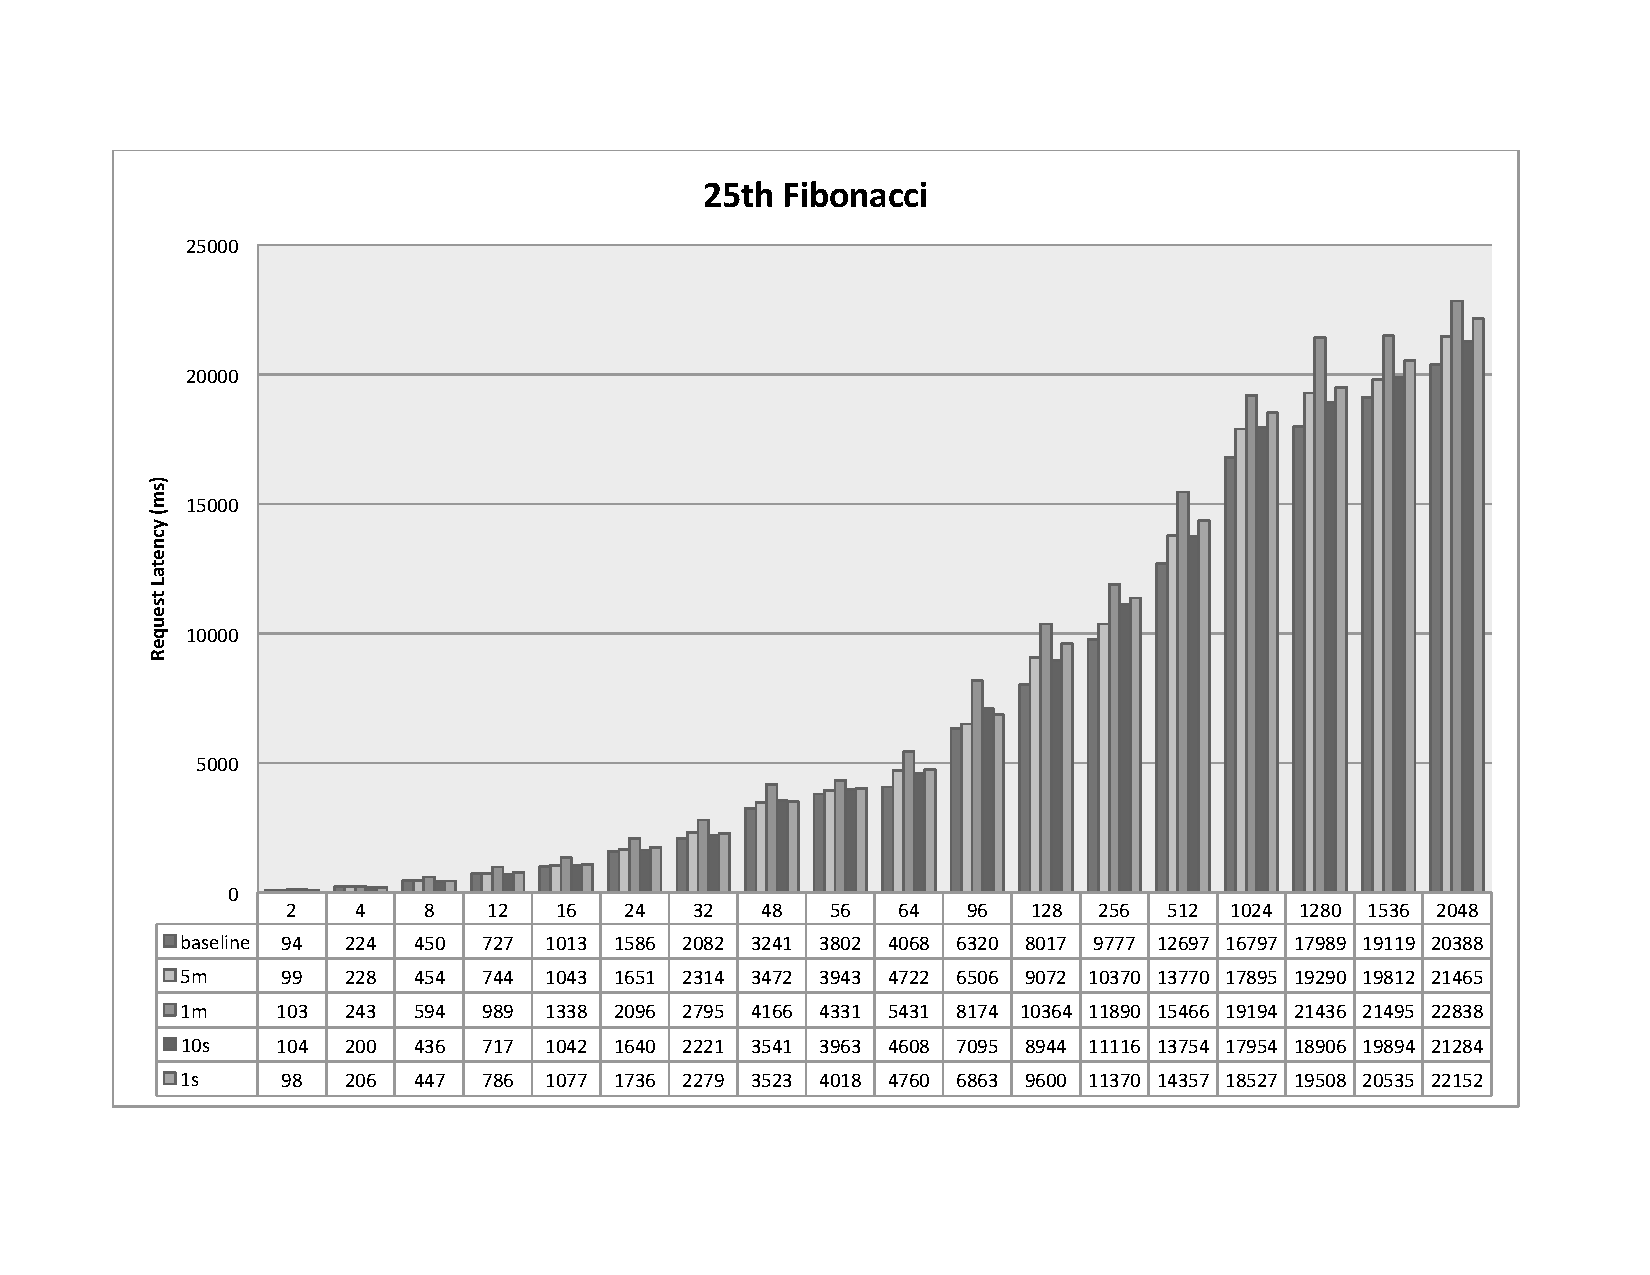
\includegraphics[scale=0.5]{compare-fib.pdf}
    \vspace{-50pt}
    \caption{25th Fibonacci Results}
    \label{fig:fib25_graph}
\end{figure}

Apache's disk-bound performance measured in the 5MB download test is relatively unaffected by \dcamp. This graph also
shows the 512 thread load point as the beginning of a trend line shift, again correlating with the increase in request
error rate.

\begin{figure}[H]
    \centering
    \vspace{-20pt}
    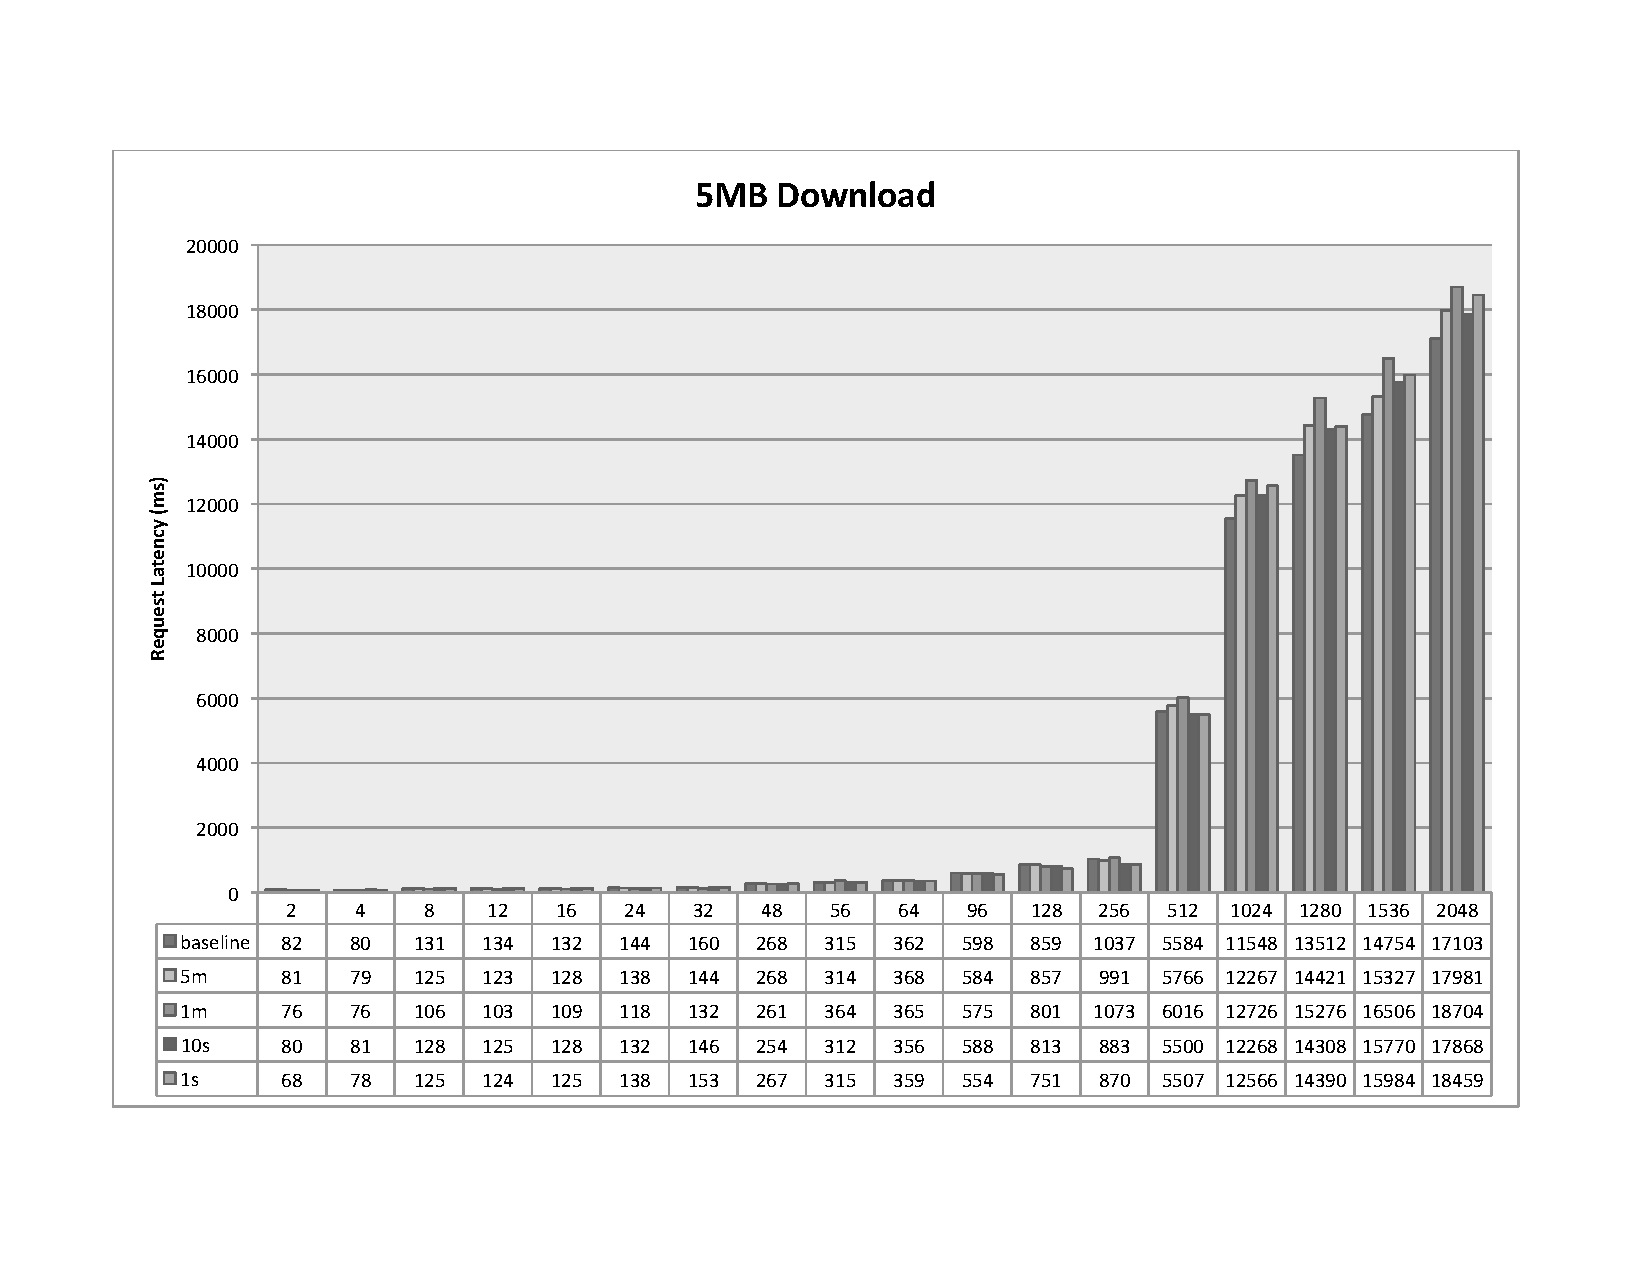
\includegraphics[scale=0.5]{compare-down.pdf}
    \vspace{-50pt}
    \caption{5MB Download Results}
    \label{fig:down5mb_graph}
\end{figure}

A few observations can be drawn from these results.

When nodes are not expected to fail frequently, using longer heartbeat periods reduces the impact \dcamp has on the
system. It is better to monitor a process using a faster sample period than an entire system using a slower sample
period. The \dcamp system impact is noticeable but a considerably smaller factor than the impact hardware limitations
have on performance monitoring.

\section{Scalability}

One of the primary measures of scalability for a distributed system is its network traffic.\cite{zanikolas2005} By
simulating successively larger \dcamp systems (with respect to node count), once can extrapolate \dcamp's effectiveness
at monitoring large distributed systems and how to best configure its metric collections.

\subsection{Workload}

\dcamp is setup to monitor a machine's global metrics, scaling the number of simulated nodes in the \dcamp system from
three nodes (one Root, one Collector, one Sensor) up to 200 nodes (eight groups with twenty-five nodes per group). The
metric configuration is kept constant for each test run. As \dcamp starts, monitors in steady state, and shuts down, the
machine's network traffic is monitored and recorded every five seconds.

The test machine is a MacBook Pro (2.7GHz Core i7, 8GB 1333MHz DDR3, SSD) running OSX 10.9. All simulated \dcamp nodes
use endpoints on the machine's loopback interface, and only the loopback interface traffic is monitored. The machine is
otherwise entirely idle during the test runs.

\subsection{\dcamp Configuration}

\dcamp is configured to monitor and report the below global metrics, using a heartbeat of 60 seconds.

\begin{itemize}
\item CPU usage every 60 seconds
\item total disk throughput every 120 seconds
\item total network throughput every 120 seconds
\item memory usage every 60 seconds
\end{itemize}

No thresholds were defined for the above configuration. That is, Sensor nodes immediately reported every sample instead
of holding them for later reporting.

\subsection{Results}

Sparklines of each load point show the same pattern: highest network traffic occurs during start up and then also on
shutdown. This pattern follows the design of \dcamp which uses a chatty configuration protocol and a terse data
protocol. The rest of steady operation shows expected low network traffic except on sample periods.

\begin{figure}[H]
    \centering
    \vspace{-20pt}
    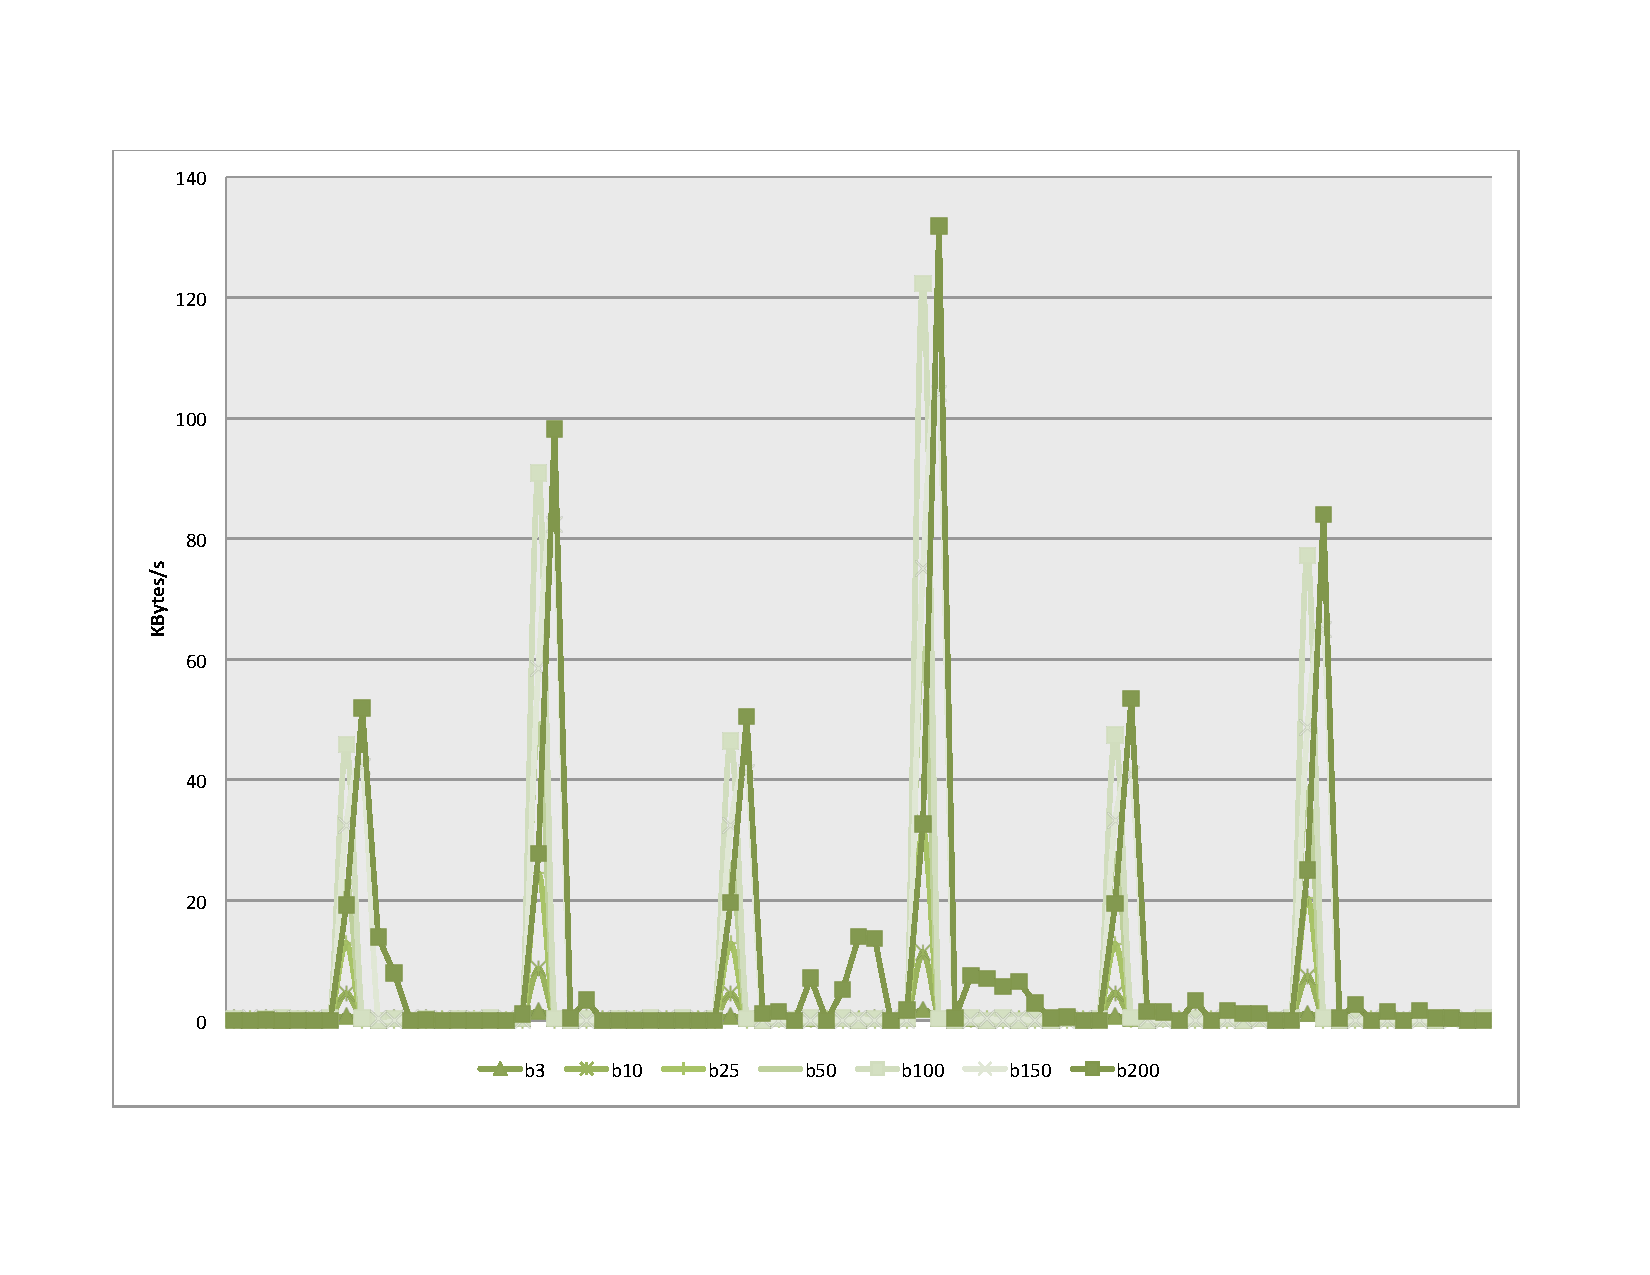
\includegraphics[scale=0.5]{dcamp-net-bytes-steady.pdf}
    \vspace{-40pt}
    \caption{Network bytes during steady operation as the number of \dcamp nodes increases.}
    \label{fig:net_bytes_steady_graph}
\end{figure}

\begin{figure}[H]
    \centering
    \vspace{-20pt}
    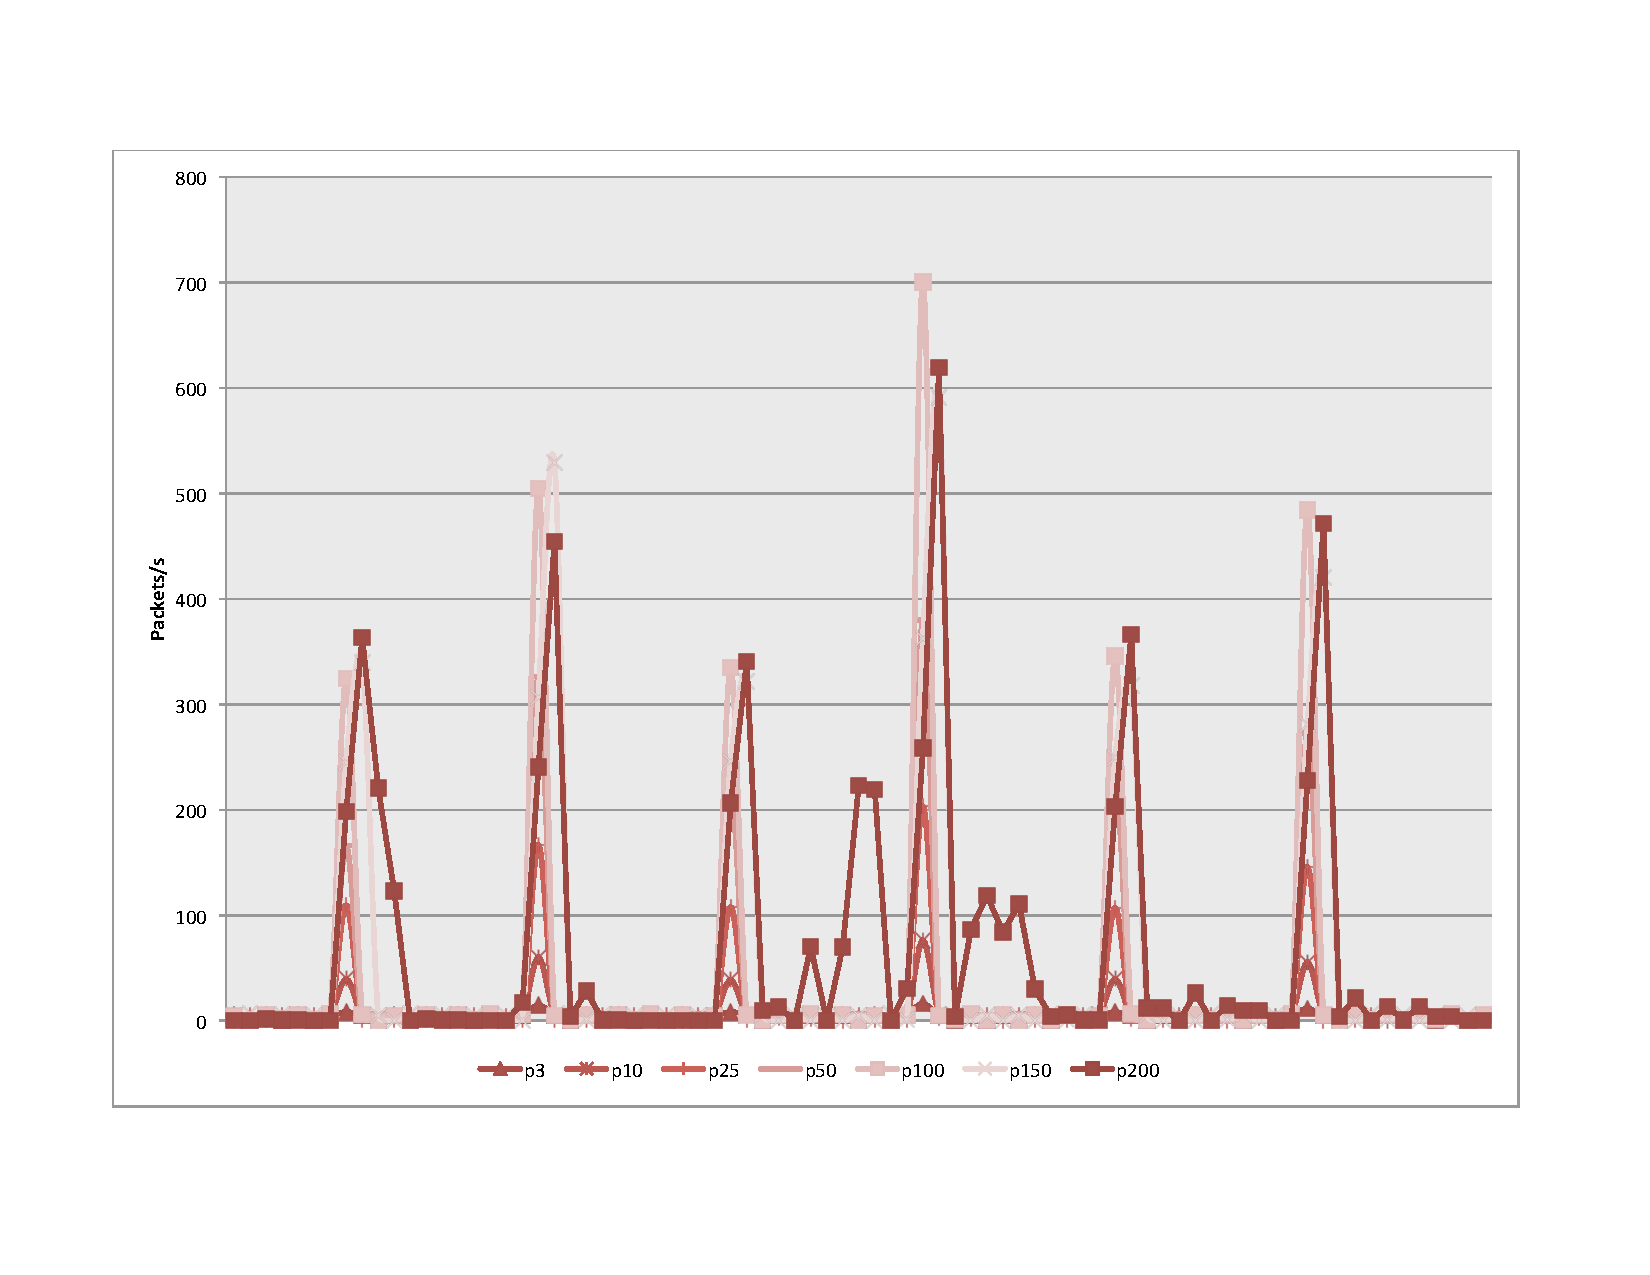
\includegraphics[scale=0.5]{dcamp-net-packets-steady.pdf}
    \vspace{-40pt}
    \caption{Network packets during steady operation as the number of \dcamp nodes increases.}
    \label{fig:net_packets_steady_graph}
\end{figure}

As the node count increases, the rate at which bytes/packets are sent and received increases. This correlates with the
larger configuration which \dcamp must track as well as the additional nodes sending and receiving data. Looking at the
same values but also relating them to the number of nodes in the system, one sees the configuration size grows faster
than the number of nodes.

However, the number of messages being sent per node actually goes down and levels off just under 1 packet per node per
second. This can be attributed to the fact that the number of Sensor nodes increases faster in relation to the number of
Collector nodes. That is, Sensor nodes do not require full-configuration replication and send/receive fewer messages
since they are relatively uninvolved with topology coordination in comparison to Collector nodes.

As this ratio increases, it is expected the number of messages per node to decrease. This latter observation indicates a
higher number of child nodes per parent would result in lower network utilization and better \dcamp scalability.

\begin{figure}[H]
    \centering
    \vspace{-20pt}
    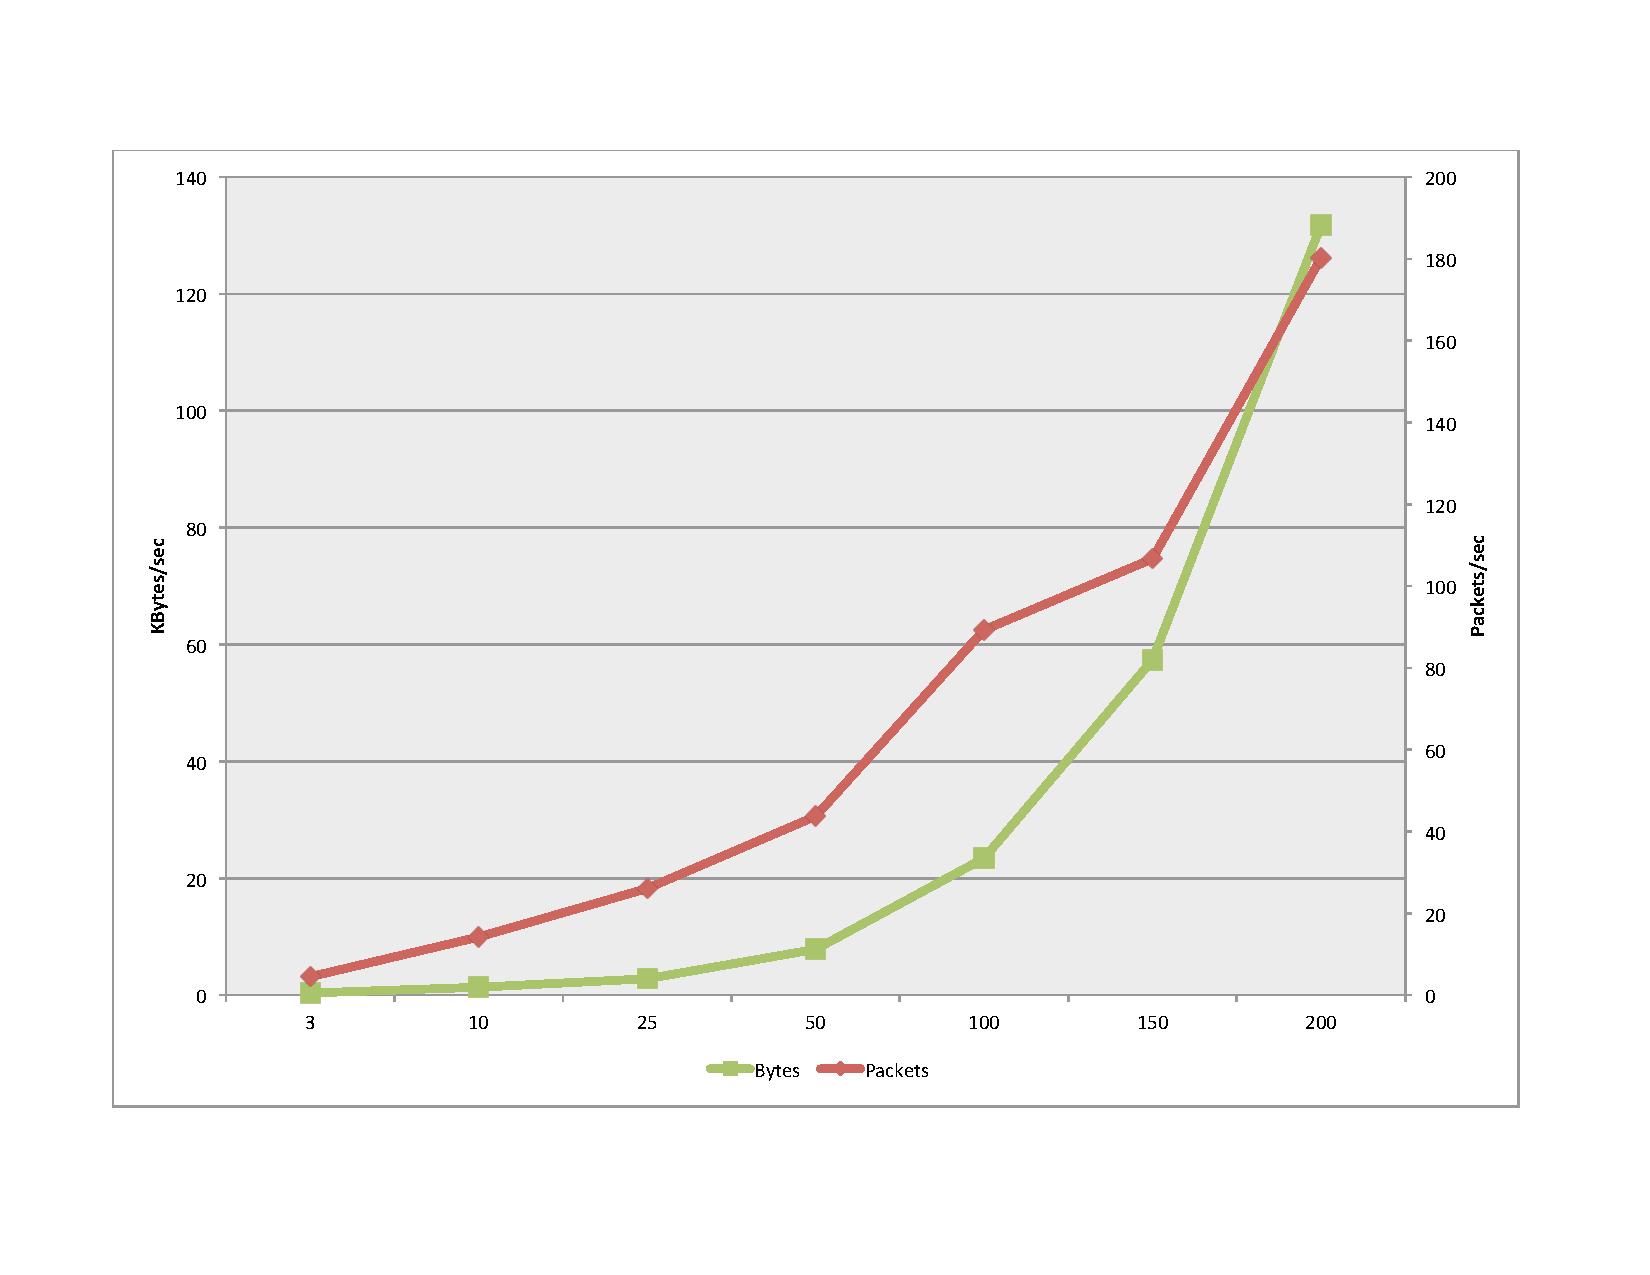
\includegraphics[scale=0.5]{dcamp-net-average.pdf}
    \vspace{-40pt}
    \caption{Average Bytes/Packets as the number of \dcamp nodes increases.}
    \label{fig:net_avg_graph}
\end{figure}

\begin{figure}[H]
    \centering
    \vspace{-20pt}
    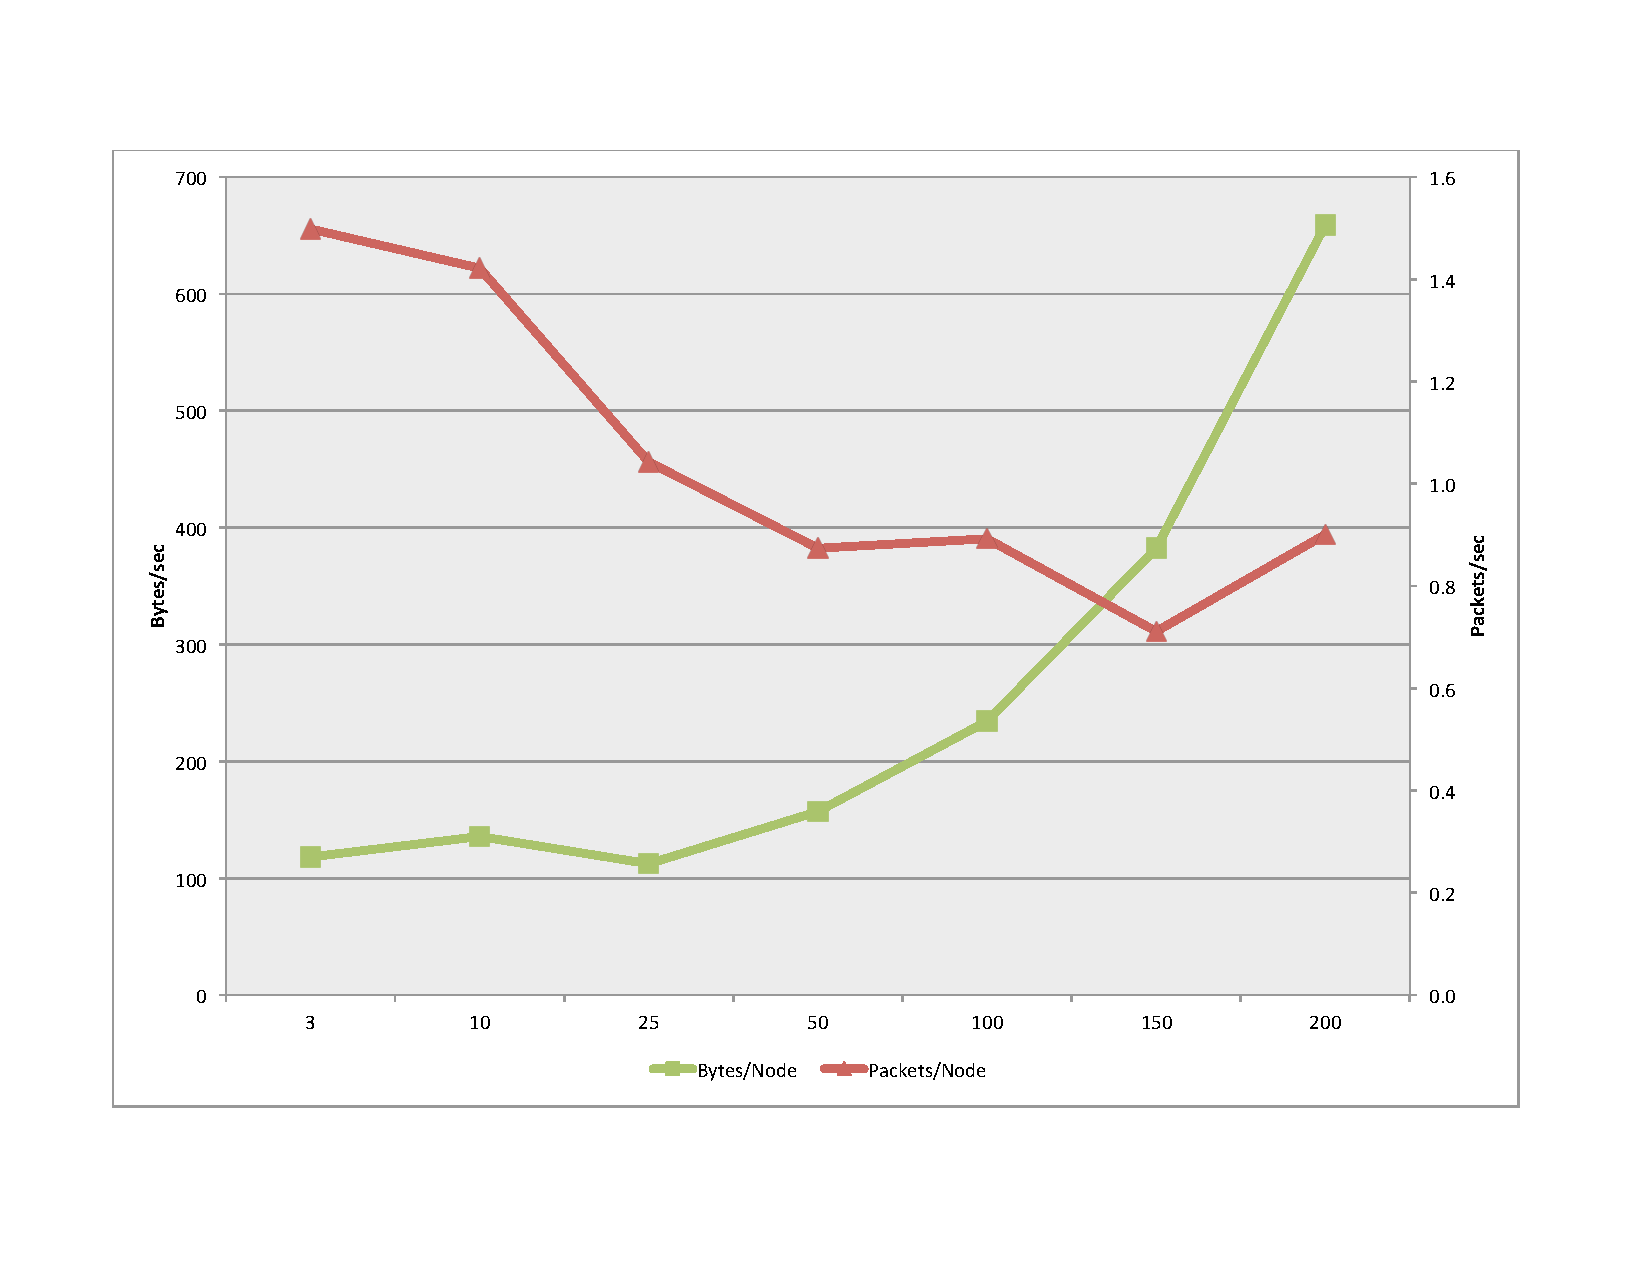
\includegraphics[scale=0.5]{dcamp-net-average-pernode.pdf}
    \vspace{-40pt}
    \caption{Average Bytes/Packets Per Node as the number of \dcamp nodes increases.}
    \label{fig:net_avg_pernode_graph}
\end{figure}

\chapter{Related Work}
\label{related_work}

\emph{THIS SECTION IS FROM MY 508 PAPER \newline AND NEEDS TO BE CLEANED UP}

Being distributed, a framework must collect data from a large number of nodes and aggregate the data to one node or client.
Implementations have been built using centralized, hierarchical, peer-to-peer and any number of other architectures.
There are three types of metric gathering techniques: (1) hardware counters and sensors use specialized hardware to gather highly accurate metrics and are highly dependent on the underlying hardware architecture, (2) software sensors use modern operating system interfaces to acquire moderately accurate performance metrics in an architecture-independent interface, and (3) hybrid approaches use a combination of hardware and software sensors to attain a balance between the two.

There are a number of distributed performance frameworks being actively researched and developed, both academically and commercially.
This work defines a set of criteria for evaluating distributed performance frameworks to measure the usefulness and viability of the framework.
In the next section I list similar survey work, showing the novelty of this paper.
Section 3 presents the evaluation criteria, section 4 provides the evaluation results of several distributed performance frameworks, and section 5 concludes.

\section{Related Work}
Several papers have been published dealing with this topic and which try to give an overview of the current state of distributed performance frameworks.
This work, while related, differs in two main aspects: (1) the evaluation criteria presented here is more complete than previous works' requirements and (2) this work looks specifically at distributed performance frameworks rather than distributed system or grid tools and frameworks.

Zoraja et al. include a section on Monitoring Issues in their work on \newline OMIS/OCM, CORAL, and MIMO \cite{zoraja1999} focusing on design and implementation issues for monitoring systems.
These monitoring issues share some critical points with the criteria presented here, but the work lacks an analysis of other distributed performance frameworks and only includes limited analysis of the presented frameworks against the listed monitoring issues.
\cite{hofmann1994} provides a short survey of related monitoring systems in comparison to the ZM4/SIMPLE monitoring environment.
While this survey does look at a number of important framework characteristics, it is restricted to hybrid distributed performance frameworks.

Allan and Ashworth published an exhaustive survey of distributed computing tools \cite{allan2001} but did not present any particular focus on distributed performance frameworks nor did they include a set of criteria for evaluating frameworks.
Zanikolas et al. present an in-depth taxonomy of grid monitoring systems \cite{zanikolas2005}, including a set of general requirements for monitoring systems.
Their work does much for defining a good set of criteria for evaluating and analyzing distributed performance frameworks, but has a much broader scope than this work.
This work expands on their monitoring system requirements to account for the completeness and validity of distributed performance frameworks.

\section{Analysis Results}
The distributed performance frameworks analyzed in this section were chosen based on their categorization in the \cite{zanikolas2005} taxonomy; only level 2 frameworks are included.
Level 2 frameworks are defined as having at least one type of republisher in addition to producers; these frameworks usually distribute functionality across multiple hosts. \cite{zanikolas2005}
A limited analysis is conducted by reviewing the available literature, and further analysis (i.e., verifying scalability, transparency, and validity) is left as future work.

\subsection{NetLogger}
Work done by Brian Tierney and Dan Gunter \cite{tierney1998} \cite{gunter2000} presents the Network Application Logger Toolkit (NetLogger).
This framework can be used to monitor the performance of distributed systems at a very detailed level.
With a new logging format and activation service \cite{gunter2002} the authors improved upon their previous work and increased the toolkit's scalability and data delivery models.
NetLogger is being actively developed and is one of the more well known distributed performance frameworks.
The toolkit is composed of four parts: an API and library for instrumenting a given application, a set of tools for collecting and sorting logs, performance sensors, and a visualization user interface for the log files.

Each part assumes the system clocks of the individual nodes are accurate and synchronized (the authors mention the use of NTP to achieve a required clock synchronization of one millisecond).
The instrumentation of code allows NetLogger to gather more detailed data from an application-to-application communication path, such as traces of network packets through a call hierarchy.
The instrumentation also allows the activation service to update the monitoring of parts of the system dynamically as consumers subscribe to various events and metrics.

Their research has shown NetLogger to be highly scalable, complete, and transparent as well as valid.
The activation service provides a push data delivery and can utilize the security mechanisms part of current web services in order to authenticate requests for performance data.
NetLogger is currently implemented for C, C++, Java, Perl, and Python applications.
Because the framework lacks black box characteristics, its portability is greatly reduced.

\subsection{JAMM}
Java Agents for Monitoring and Management (JAMM) \cite{tierney2000} is the fruit of work by the authors of NetLogger to build a monitoring system with managed sensors. 

The JAMM system consists of six components: sensors, sensor managers, event gateways, directory service, event consumers, and event archives.
There is a sensor manager on each host, with the sensors acting as producers for the gateways which they publish the data to.
The gateways can then filter and aggregate the incoming data according to consumer queries.
The directory service is used to publish the location of the sensors and gateways, allowing for dynamic discovery of active sensors by the consumers.
The event archive is used for historical analysis purposes.

JAMM explicitly uses a pull data delivery model where data is only sent when requested by a consumer.
The overall architecture is generally distributed with the directory service being centralized.
JAMM, being heavily based off of NetLogger, inherits the validity, completeness, security, and transparency of NetLogger along with its lack of portability.
JAMM does, however, prove itself in terms of scalability with it's own architecture.

\subsection{Hawkeye}
Hawkeye \cite{hawkeye} is a monitoring and management tool for distributed systems which makes use of technology previously researched and developed as part of the Condor project \cite{litzkow1988}.
Condor provides mechanisms for collecting information about large distributed computer systems.
Hawkeye is being readily developed and is freely available for download on Linux and Solaris.

Hawkeye uses a general push delivery model by configuring Condor to execute programs, or modules, at given time intervals, collect performance data, and send it to the central manager.
These modules are configurable such that the "period' of module execution can be set to a given time frame in seconds, minutes, or hours or the module can be executed in "continuous" mode where the module's execution never ends.
The available modules for monitoring a Condor pool include: disk space, memory used, network errors, open files, CPU monitoring, system load, users, Condor Node, Condor Pool, and Grid Probe.
Custom modules can also be developed and installed for monitoring of arbitrary resources and metrics.
Data can be accessed from the central manager via an API, CLI, or GUI.

While no experiments have been run, the generally centralized manager reduces the Hawkeye framework's scalability, and its transparency is unknown.
The frameworks module based producer architecture gives it an infinite completeness, but being only available on Linux and Solaris makes the framework less portable.
Lastly, the ability to run jobs securely on target machines has been left as future work by the authors.

\subsection{SCALEA-G}
Truong and Fahringer present SCALEA-G \cite{truong2004}, an unified monitoring and performance analysis system for distributed systems.
It is based on the Open Grid Service Architecture \cite{foster2002} and allows for a number of services to monitor both grid resources and grid application.
SCALEA-G uses dynamic instrumentation to profile and trace Java and C/C++ applications in both push and pull data delivery models, making the framework both scalable and portable.

The SCALEA-G framework is composed of several services: directory service, archival service, sensor manager service, instrumentation service, client service, and user portal.
These services provide the following functionality respectively: publishing and searching of producers and consumers, storage of performance results, management of sensors, dynamic instrumentation of source code, administering clients and analyzing data, and on-line monitoring and performance analysis.

The framework makes use of secure sockets to achieve secure communications and achieves high completeness via code instrumentation.
Unfortunately, the authors do not provide any report on SCALEA-G's validity or transparency.

\subsection{IMPuLSE}
Integrated Monitoring and Profiling for Large Scale Environments \cite{bridges2004} was designed to address "operating system-induced performance anomalies" and provide "accurate, low-overhead, whole-system monitoring." The authors have chosen to develop a message-centric approach which associates data with messages rather than hosts and a system-wide statistical sampling to increases the framework's scalability.

The IMPuLSE framework is still in the design stage, and therefore lacks any implementation data outside of their new message-centric design pattern which shows promising results.
Unfortunately, this leaves the framework with unknown transparency, security, completeness, portability, and validity.

\section{Conclusion}
There are a number of high quality and effective distributed performance frameworks being actively researched and developed, but with some frameworks having more research than others, there is a natural disparity of information about each framework.
While the frameworks vary in distributed architecture and features, they all fulfill the minimum requirements of performance frameworks.
The frameworks analyzed in this work are mainly software based sensor frameworks.
This was chosen due to the inherent portability advantage of software sensors over hardware or hybrid sensors.

Many authors have failed to address their framework's validity, transparency, and scalability explicitly, thinking the framework's architecture speaks for itself or blindly assuming it is accurate and introduces negligible load on the measured system.
I leave it as future work to conduct formal experiments to test validity, transparency, and scalability of the distributed performance frameworks analyzed here.


\chapter{Future Work}
\label{future_work}

\begin{itemize}

\item uniform configuration: The configuration of the entire system is uniform, i.e., all branches of the system will be
collecting the same data at each level in the hierarchy---it is not possible to have different data being collected by
different branches.

\item network failure: \dcamp does not support any fault tolerance for network failures; \dcamp only attempts to recover
from node failures. It is assumed that if (part of) the network goes down, the lack of data from that subnet will
suffice

\item time accuracy: The system time among multiple nodes in the system may vary significantly; \dcamp is not meant to
be a high-resolution system with respect to the order of performance data occurrences. It is assumed that the ordering
of performance events in the system is insignificant and timestamps associated with performance data are rough
estimates.

\end{itemize}


\chapter{Conclusions}
\label{conclusions}

\section{Summary of Contributions}

\section{Future Work}
\label{future_work}
\chapter{Future Work}
\label{future_work}

\subsubsection{Additional Features}

While \dcamp in its current implementation meets the requirements of a basic DPF, these features should advance it into
a more complete, end-to-end distributed performance monitoring solution.

An \textbf{end-to-end tool} built on top of \dcamp could allow a system administrator to quickly look at the performance
of a large part of the network via aggregate metrics and easily drill down into the groups and/or nodes which exhibit
problematic behaviour. Toward this goal, a \textbf{lightweight web server} could be implemented on each node, adding
support for REST APIs and access to historical metric data along with a graphical user interface for easier \dcamp
system management.

The current \dcamp protocols leave much to be desired when it comes to secure communication and operation. A more secure
implementation would include a form of \textbf{salted pass phrases} with every control message or even encrypt all
messages sent from one node to another.

One of the possible pain points with \dcamp is the control given to the system administrator through group
specifications. Specifically, administrators are tasked not only with identifying which nodes to include in the system,
but also how those nodes are placed into the distributed topology. Instead of this manual configuration,
\textbf{automatic grouping} of nodes may be implemented based on network locality, metric configuration and sample
periods, or even a tunable such as preference of network vs. CPU/memory overhead. The administrator would be left with
the task of defining which metrics a given node should collect and \dcamp would best select where the nodes sit in the
hierarchy, how many children nodes a single parent manages, etc.

\subsubsection{Fault Tolerance}

The fault tolerance of \dcamp could be improved by implementing these features which were considered out-of-scope for
the original project.

\dcamp does not support any fault tolerance for network failures---it only attempts to recover from node failures. It is
assumed that if (part of) the network goes down, the lack of data from that subnet will suffice. Specifically, \dcamp
cannot currently tolerate a \textbf{split-brain syndrome} in which the network has been partitioned and entire subsets
of the system cannot communicate with each other. It may be enhanced to recover from such network partitions, though.

The system time among multiple nodes in the distributed system may vary significantly. \dcamp is not meant to be a
high-resolution system with respect to the \textbf{ordering of performance data occurrences}. It is assumed that NTP
provides sufficient time synchronization across all nodes in the system OR the precise ordering of performance events in
the system is not required.

To further increase fault tolerance of the topology, \dcamp should be able to \textbf{operate without a \textit{Root}}
node. That is, the Management service should not be continuously needed for the system to operate. Essentially this
comes down to all top-level \textit{Collector} nodes being potential endpoints for end-user control, at which point it
momentarily acts as a Root, sending out configuration updates.

Lastly, as described in Chapter \ref{implementation}, \dcamp could become more resilient to software failures by running
\textit{Base} nodes within a \textbf{self-restarting executable}. If the process crashes for any reason, it would
automatically be restarted and join back into the network.

\subsubsection{Improve Performance and Scalability}

With several places for improvement, increasing the efficiency and performance of \dcampns's own implementation could
make really large systems feasible.

The current implementation of each ZeroMQ protocol heavily relies on a common polling pattern. Not only does this waste
thread resources waiting on socket connections, but the code becomes hard to maintain as well. An alternate solution to
this polling is event-driven I/O. ZeroMQ supports this alternate messaging pattern via Facebook's \textbf{Tornado
IOLoop}\cite{tornado}\cite{ioloop} and libev via \textbf{gevent}\cite{gevent}\cite{libev}.

With IOLoop, it may be possible to use a single IO loop, hosted by the \textit{Base} node, shared among all the active
services. This reduces the number of idle threads per node, freeing valuable operating system resources and reducing
\dcampns's processing overhead.

Although \dcamp only uses classic TCP protocols for all communication, ZeroMQ does support \textbf{multicast network
protocols}. Using multicast judiciously within \dcamp could greatly reduce configuration costs and network traffic, for
example in the \hyperref[proto_topo]{Topology Protocols}. For \dcamp systems spanning multiple subnets, the use of
multicast would require special network configurations or special ZeroMQ gateways for passing messages from one subnet
to the next.

\textbf{Multiple-level branches} are not supported in the current implementation. That is, all \textit{Collector} nodes
have the \textit{Root} node as their parent and only have \textit{Metric} nodes as their children. Extending support for
multiple levels of \textit{Collectors} would allow large group configurations to be automatically split into multiple
(identically configured) branches for improved scalability

Compiling the various critical paths within \dcampns, such as the metric sampling code in the Sensor service, using
\textbf{Pyrex}\cite{pyrex} or \textbf{Cython}\cite{cython} may boost performance and lower the cost of metric collection
such that faster sample periods can be used without issue.

Due to Python's Global Interpreter Lock\cite{py-threads}, there are limitations to the parallel execution of threads on
an SMP system. While \dcampns's use of threads is heavily I/O-bound, some gains may also be found by using full-fledged
\textbf{processes instead of threads}.

While not a huge cost, \dcamp currently requires two nodes to execute alongside each other on a system which hosts a
\textit{Collector}. An improvement would be to provide full support for \textbf{metric sampling directly within the
\textit{Collector} role}.

\subsubsection{Metric Extensions}

Only a small subset of metrics were implemented in \dcamp as a proof of concept. The rest of the full set listed in the
\hyperref[dcamp_metrics]{\dcamp Metrics} section are left as future work.

Beyond the list of statically defined metrics, \textbf{user-defined metrics} would expand the performance monitoring
infinitely. This could be implemented as a Python module integrated into the distributed system being monitored or
through a plug-in system built into \dcamp itself.

Additionally, \dcamp could support additional data types such as \textbf{histograms} and \textbf{variable length
strings} or even more fine grained control over when metrics are sampled. For example, metrics could be
\textbf{collected on demand}, driven by user requests via the Management service, or collected at a special ``once''
sample period so data is sent to the \textit{Root} node only at start.

There are also two features which can be implemented to improve collection and reporting efficiency. First, a more
compact data message format could be used to \textbf{combine multiple data samples into a single message}, e.g. for
aggregation purposes or representing entire branches in the topology. This would improve network efficiency as fewer
packets would require routing and data could be more effectively compressed. Second, metrics could be sampled regularly
but \textbf{reported randomly} within the period in order to distribute arrival of data from child nodes and not
overload the Aggregation service.

Lastly, \dcamp could be extended to support some hardware performance counters, bringing it more in-line with hybrid
performance frameworks. In particular, it would be interesting to add support for Graphical Processing Unit metrics such
as those available via the NVIDIA Management Library\cite{nvidiaML} which already has Python bindings support
\cite{py-nvidia}.



% ------------- End main chapters ----------------------

\clearpage

\bibliography{refs}
\bibliographystyle{abbrv}

\appendix
\chapter{ZeroMQ Primer}
\label{zeromq_primer}

\section{Socket Types and Message Patterns}

\begin{itemize}

\item PUB/SUB

\item REQ/REP

\item PUSH/PULL

\end{itemize}

\chapter{Completing a Thesis in the Real World}
\label{get_it_done}

Do not waste your time.
Real life is full of real work. Marriage. Babies.
Life is not waiting.



\end{document}

